\documentclass[fleqn, a4paper, 12pt, twoside]{article}

\newcounter{recitationcount} %creates a new counter for recitation numbers (must be executed before exsheets is loaded)
\newcommand\recitation{\refstepcounter{recitationcount}}

\usepackage[counter-within = recitationcount]{exsheets} %question and solution environments
\usepackage{amsmath, amssymb, amsthm} %standard AMS packages
\usepackage{esint} %integral signs
\usepackage{marginnote} %marginnotes
\usepackage{gensymb} %miscellaneous symbols
\usepackage{commath} %differential symbols
\usepackage{xcolor} %colours
\usepackage{cancel} %cancelling terms
\usepackage[free-standing-units]{siunitx} %formatting units
\usepackage{tikz, pgfplots} %diagrams
	\usetikzlibrary{calc, hobby, patterns, intersections, angles, quotes, spy}
\usepackage{graphicx} %inserting graphics
\usepackage{epstopdf} %converting and inserting eps graphics
\usepackage{hyperref} %hyperlinks
\usepackage{datetime} %date and time
\usepackage{ulem} %underline for \emph{}
\usepackage{xfrac, lmodern} %inline fractions
\usepackage{enumerate, enumitem} %numbered lists
\usepackage{float} %inserting floats
\usepackage[american voltages]{circuitikz} %circuit diagrams
\usepackage{pdflscape} %pages in landscape orientation
\usepackage{setspace} %double spacing
\usepackage{microtype} %micro-typography
\usepackage{listings} %formatting code
	\lstset{language=Matlab}
	\lstdefinestyle{standardMatlab}
	{
		belowcaptionskip=1\baselineskip,
		breaklines=true,
		frame=L,
		xleftmargin=\parindent,
		language=C,
		showstringspaces=false,
		basicstyle=\footnotesize\ttfamily,
		keywordstyle=\bfseries\color{green!40!black},
		commentstyle=\itshape\color{purple!40!black},
		identifierstyle=\color{blue},
		stringstyle=\color{orange},
	}
\usepackage{algpseudocode} %algorithms
\usepackage{algorithm} %algorithms

\renewcommand{\marginfont}{\scriptsize \color{blue}}

\newcommand\numberthis{\addtocounter{equation}{1}\tag{\theequation}} %adds numbers to specific equations in non-numbered list of equations

\theoremstyle{definition}
\newtheorem{example}{Example}
\newtheorem{definition}{Definition}

\theoremstyle{theorem}
\newtheorem{theorem}{Theorem}
\newtheorem{law}{Law}

\newcommand{\curl}{\mathrm{curl\,}}

\newcommand{\divergence}{\mathrm{div\,}}

\makeatletter
\@addtoreset{section}{part} %resets section numbers in new part
\makeatother

\newcommand\blfootnote[1]{%
	\begingroup
	\renewcommand\thefootnote{}\footnote{#1}%
	\addtocounter{footnote}{-1}%
	\endgroup
}

\renewcommand{\tilde}{\widetilde}

\RenewQuSolPair{question}[name=Recitation \therecitationcount\ -- Exercise]{solution}[name=Recitation \therecitationcount\ -- Solution]

\SetupExSheets{solution/print = true} %prints all solutions by default

%opening
\title{Harmonic Analysis : Recitations}
\author{Aakash Jog}
\date{2015-16}

\begin{document}

\maketitle
%\setlength{\mathindent}{0pt}

\blfootnote
{	
	\begin{figure}[H]
		
\includegraphics[height = 12pt]{cc.eps}
		\includegraphics[height = 12pt]{by.eps}
		\includegraphics[height = 12pt]{nc.eps}
		\includegraphics[height = 12pt]{sa.eps}
	\end{figure}
	This work is licensed under the Creative Commons Attribution-NonCommercial-ShareAlike 4.0 International License. To view a copy of this license, visit \url{http://creativecommons.org/licenses/by-nc-sa/4.0/}.
} %CC-BY-NC-SA license

\tableofcontents

\newpage
\section{Instructor Information}

\textbf{Yaron Yeger}\\
~\\
Office: Shenkar Physics 201\\
E-mail: \href{mailto:yaronyeg@mail.tau.ac.il}{yaronyeg@mail.tau.ac.il}\\

\newpage
\part{Fourier Series}

\recitation
\section{Fourier Series}

\begin{definition}[Real Fourier series]
	Let $f : [-L,L] \in \mathbb{C}$ be a piecewise continuous function.\\
	The series
	\begin{align*}
		f(x) & \approx \frac{a_0}{2} + \sum\limits_{n = 1}^{\infty} \left( a_n \cos(n x) + b_n \sin(n x) \right)
	\end{align*}
	is called the Fourier series of $f(x)$, where
	\begin{align*}
		a_0 & = \frac{1}{L} \int\limits_{-L}^{L} f(x) \dif x           \\
		a_n & = \frac{1}{L} \int\limits_{-L}^{L} f(x) \cos(n x) \dif x \\
		b_n & = \frac{1}{L} \int\limits_{-L}^{L} f(x) \sin(n x) \dif x
	\end{align*}
\end{definition}

\begin{theorem}
	If $f(x)$ is an even function, then the appropriate Fourier series is
	\begin{align*}
		f(x) & \approx \frac{a_0}{2} + \sum\limits_{n = 1}^{\infty} a_n \cos(n x)
	\end{align*}
	If $f(x)$ is an odd function, then the appropriate Fourier series is
	\marginnote
	{
		If $f(x)$ is odd, its graph always passes through the origin.
		Therefore, it can be represented by a summation of sine functions, which also pass through the origin, and there is no need for a term, i.e. $\frac{a_0}{2}$, to change its position at the origin.
	}
	\begin{align*}
		f(x) & \approx \sum\limits_{n = 1}^{\infty} a_n \sin(n x)
	\end{align*}
\end{theorem}

\begin{definition}[Complex Fourier series]
	Let $f : [-L,L] \in \mathbb{C}$ be a piecewise continuous function.\\
	The series
	\begin{align*}
		f(x) & \approx \sum\limits_{n = -\infty}^{\infty} c_n e^{i n x}
	\end{align*}
	is called the complex Fourier series of $f(x)$, where
	\begin{align*}
		c_n & = \frac{1}{2 L} \int\limits_{-L}^{L} f(x) e^{-i n x} \dif x
	\end{align*}
\end{definition}

\begin{question}
	Calculate the real Fourier series of
	\begin{align*}
		f(x) & = 2 x - 2 \pi
	\end{align*}
\end{question}

\begin{solution}
	As $x$ is an odd function, the real Fourier series of $x$, in the interval $[-\pi,\pi]$ is
	\begin{align*}
		x & \approx \sum\limits_{n = 1}^{\infty} b_n \sin(n x)
	\end{align*}
	where
	\begin{align*}
		b_n & = \frac{1}{\pi} \int\limits_{-\pi}^{\pi} x \sin(n x) \dif x                                                                                                   \\
                    & = \frac{1}{\pi} \left. \left( x \int \sin(n x) \dif x - \int 1 \left( \int \sin(n x) \dif x \right) \dif x \right) \right|_{-\pi}^{\pi}                      \\
                    & = \frac{1}{\pi} \left. \left( -\frac{x \cos(n x)}{n} \right) \right|_{-\pi}^{\pi} + \frac{1}{\pi} \int\limits_{-\pi}^{\pi} \frac{\cos(n x)}{n} \dif x        \\
                    & = \frac{1}{\pi} \left( -\frac{\pi \cos(n \pi) + \pi \cos(-n \pi)}{n} \right) + \frac{1}{\pi} \cancelto{0}{\left. \frac{\sin(n x)}{n^2} \right|_{-\pi}^{\pi}} \\
                    & = -\frac{\cos(n \pi) + \cos(n \pi)}{n}                                                                                                                       \\
                    & = -2 \frac{\cos(n \pi)}{n}                                                                                                                                   \\
                    & = -2 \frac{(-1)^{n}}{n}
	\end{align*}
	Therefore,
	\begin{align*}
		x & \approx 2 \sum\limits_{n = 1}^{\infty} \frac{(-1)^{n + 1}}{n} \sin(n x)
	\end{align*}
	Therefore,
	\begin{align*}
		2 x - 2 \pi & \approx \left( 4 \sum\limits_{n = 1}^{\infty} \frac{(-1)^{n + 1}}{n} \sin(n x) \right) - 2 \pi \\
	\end{align*}
\end{solution}

\recitation
\section{Bessel's Inequality}

\begin{definition}[Piecewise continuous functions]
	$f : \mathbb{R} \to \mathbb{R}$ is said to be piecewise continuous if, for every finite interval $[a,b]$ there is a finite number of discontinuity points, and the one-sided limits at each of these points are also finite.
\end{definition}

\begin{definition}[Piecewise continuously differentiable functions]
	$f : \mathbb{R} \to \mathbb{R}$ is said to be piecewise continuously differentiable if it is piecewise continuous, and
	\begin{align*}
		\lim\limits_{h \to 0^+} \frac{f(x + h) - f(x^+)}{h} & < \infty
	\end{align*}
	and
	\begin{align*}
		\lim\limits_{h \to 0^-} \frac{f(x + h) - f(x^-)}{h} & < \infty
	\end{align*}
\end{definition}

\begin{theorem}[Bessel's Inequality]
	Let $f(x)$ be a piecewise continuous function defined on $[-L,L]$.
	Then
	\begin{align*}
		\frac{1}{2} {a_0}^2 + \sum\limits_{n = 1}^{\infty} {a_n}^2 + {b_n}^2 & \le \frac{1}{L} \int\limits_{-L}^{L} {f(x)}^2 \dif x
	\end{align*}
	\label{Bessel's_Inequality}
\end{theorem}

\section{Riemann-Lebesgue's Lemma}

\begin{theorem}[Riemann-Lebesgue's Lemma]
	If $f(x)$ is piecewise continuous on $[-L,L]$, then
	\begin{equation*}
		\lim\limits_{n \to \infty} a_n = \lim\limits_{n \to \infty} b_n = 0
	\end{equation*}
	\label{Riemann-Lebesgue's_Lemma}
\end{theorem}

\section{Dirichlet's Kernel}

\begin{definition}[Dirichlet kernel]
	\begin{align*}
		D_m(t) & = \frac{1}{2} \sum\limits_{n = -m}^{m} e^{-i n t} \\
                       & = \frac{1}{2} + \sum\limits_{n = 1}^{m} \cos(n t) \\
                       & = \frac{\sin\left( \left( n + \frac{1}{2} \right) t \right)}{2 \sin \frac{t}{2}}
	\end{align*}
	is called the Dirichlet kernel of order $m$.
\end{definition}

\begin{theorem}[Second representation of Dirichlet's kernel]
	Let $m \in \mathbb{N}$.\\
	Then, for $t \neq 2 \pi k$, where $k \in \mathbb{Z}$,
	\begin{align*}
		D_m(t) & = \frac{1}{2} + \cos(t) + \cos(2 t) + \dots + \cos(m t) \\
                       & = \frac{\sin\left( \left( m + \frac{1}{2} \right) t \right)}{2 \sin\left( \frac{1}{2} t \right)}
	\end{align*}
\end{theorem}

\begin{theorem}
	Let
	\begin{align*}
		S_m(f,x) & = \frac{1}{2} a_0 + \sum\limits_{n = 1}^{m} a_n \cos(n x) + b_n \sin(n x)
	\end{align*}
	Then,
	\begin{align*}
		S_m(f,x) & = \frac{1}{\pi} \int\limits_{-\pi}^{\pi} f(x + t) \left( \frac{1}{2} \sum\limits_{n = 1}^{m} \cos(n t) \right) \dif t
	\end{align*}
\end{theorem}

\begin{theorem}[Dirichlet Theorem]
	Let $f : [-\pi,\pi] \to \mathbb{R}$ be a piecewise continuously differentiable function.\\
	Then, $\forall x \in (-\pi,\pi)$,
	\begin{align*}
		\frac{1}{2} a_0 + \sum\limits_{n = 1}^{\infty} a_n \cos(n x) + b_n \sin(n x) & = \frac{f(x^-) + f(x^+)}{2}
	\end{align*}
	and for $x = \pi$ or $x = -\pi$,
	\begin{align*}
		\frac{1}{2} a_0 + \sum\limits_{n = 1}^{\infty} a_n \cos(n x) + b_n \sin(n x) & = \frac{f(\pi^-) + f(-\pi^+)}{2}
	\end{align*}
	\label{Dirichlet_Theorem}
\end{theorem}

\begin{question}
	The Fourier series of $x^2$ of given to be
	\begin{align*}
		x^2 & \approx \frac{\pi^2}{3} + 4 \sum\limits_{n = 1}^{\infty} \frac{(-1)^n}{n^2} \cos(n x)
	\end{align*}
	Calculate
	\begin{align*}
		\sum\limits_{n = 1}^{\infty} \frac{1}{n^2}
	\end{align*}
\end{question}

\begin{solution}
	As $x^2$ is continuous, with a continuous derivative, \nameref{Dirichlet_Theorem} is applicable.\\
	Therefore, let
	\begin{align*}
		x & = \pi
	\end{align*}
	Therefore, by \nameref{Dirichlet_Theorem},
	\begin{align*}
		\frac{\pi^2}{3} + 4 \sum\limits_{n = 1}^{\infty} \frac{(-1)^n}{n^2} \cos(n x)         & = \frac{\left( \pi^- \right)^2 + \left( \left( -\pi \right)^+ \right)^2}{2} \\
		\therefore \frac{\pi^2}{3} + 4 \sum\limits_{n = 1}^{\infty} \frac{(-1)^n}{n^2} (-1)^n & = \pi^2                                                                     \\
		\therefore \frac{\pi^2}{4} + 4 \sum\limits_{n = 1}^{\infty} \frac{1}{n^2}             & = \pi^2                                                                     \\
		\therefore \sum\limits_{n = 1}^{\infty} \frac{1}{n^2}                                 & = \frac{1}{4} \left( \pi^2 - \frac{\pi^2}{3} \right)                        \\
                                                                                                      & = \frac{\pi^2}{6}
	\end{align*}
\end{solution}

\begin{question}
	The Fourier series of
	\begin{align*}
		f(x) &=
			\begin{cases}
				x & ;\quad 0 \le x \le \pi  \\
				0 & ;\quad -\pi \le x \le 0 \\
			\end{cases}
	\end{align*}
	is given to be
	\begin{align*}
		f(x) & \approx \frac{\pi}{4} + \sum\limits_{n = 1}^{\infty} \left( \frac{(-1)^{n + 1}}{n} \sin(n x) - \frac{2}{\pi (2 n - 1)^2} \cos\left( (2 n - 1) x \right) \right)
	\end{align*}
	Let this Fourier series be denoted by $S(x)$.\\
	Calculate
	\begin{enumerate}
		\item $1 + \frac{1}{3^2} + \frac{1}{5^2} + \dots$
		\item $S\left( \frac{\pi}{2} \right)$
	\end{enumerate}
\end{question}

\begin{solution}
	\begin{enumerate}[leftmargin=*]
		\item
			\begin{align*}
				1 + \frac{1}{3^2} + \frac{1}{5^2} + \dots & = \sum\limits_{n = 1}^{\infty} \frac{1}{(2 n - 1)^2}
			\end{align*}
			Therefore, for $x = 0$, by \nameref{Dirichlet_Theorem},
			\begin{align*}
				\frac{\pi}{4} + \sum\limits_{n = 1}^{\infty} \left( \frac{(-1)^{n + 1}}{n} \sin(0) - \frac{2}{\pi (2 n - 1)^2} \cos(0) \right) & = \frac{f(0^-) + f(0^+)}{2} \\
				\therefore \frac{\pi}{4} - \sum\limits_{n = 1}^{\infty} \left( \frac{2}{\pi (2 n - 1)^2} \right)                               & = 0                         \\
				\therefore \frac{\pi}{4} - \frac{2}{\pi} \sum\limits_{n = 1}^{\infty} \left( \frac{1}{(2 n - 1)^2} \right)                     & = 0                         \\
				\therefore \sum\limits_{n = 1}^{\infty} \frac{1}{(2 n - 1)^2}                                                                  & = \frac{\pi^2}{8}
			\end{align*}
		\item
			By \nameref{Dirichlet_Theorem},
			\begin{align*}
				S\left( \frac{\pi}{2} \right) & = \frac{f\left( {\frac{\pi}{2}}^- \right) + f\left( {\frac{\pi}{2}}^+ \right)}{2} \\
                                                              & = \frac{\pi}{2}
			\end{align*}
	\end{enumerate}
\end{solution}

\recitation

\begin{theorem}
	If $f$ is a piecewise continuous and periodic function with period of $2 \pi$, then
	\begin{align*}
		S_m(x) & = \frac{a_0}{2} + \sum\limits_{n = 1}^{m} \left( a_n \cos(n x) + b_n \sin(n x) \right) \\
                       & = \frac{1}{\pi} \int\limits_{-\pi}^{\pi} f(x + t) D_m(t) \dif t
	\end{align*}
\end{theorem}

\begin{question}
	Calculate the limit
	\begin{align*}
		L & = \lim\limits_{n \to \infty} \int\limits_{-n}^{n} \sin\left( \frac{2 n + 1}{2} t \right) \frac{\cos^2\left( \frac{\pi}{4} + t \right) + \pi^2}{\sin\left( \frac{t}{2} \right)} \dif t
	\end{align*}
\end{question}

\begin{solution}
	\begin{align*}
		L & = \lim\limits_{n \to \infty} \int\limits_{-n}^{n} \sin\left( \frac{2 n + 1}{2} t \right) \frac{\cos^2\left( \frac{\pi}{4} + t \right) + \pi^2}{\sin\left( \frac{t}{2} \right)} \dif t                      \\
                  & = 2 \lim\limits_{n \to \infty} \int\limits_{-\pi}^{\pi} \left( \cos^2\left( \frac{\pi}{4} + t \right) + \pi^2 \right) \frac{\sin\left( n + \frac{1}{2} t \right)}{2 \sin\left( \frac{t}{2} \right)} \dif t \\
                  & = 2 \lim\limits_{n \to \infty} \int\limits_{-\pi}^{\pi} \left( \cos^2\left( \frac{\pi}{4} + t \right) + \pi^2 \right) D_n(t) \dif t
	\end{align*}
	Let
	\begin{align*}
		f(x) & = \cos^2 x + \pi^2
	\end{align*}
	Let $S_n$ be the partial sum of the Fourier series.\\
	Therefore,
	\begin{align*}
		S_n & = \frac{1}{\pi} \int\limits_{-\pi}^{\pi} D_n(t) \left( \cos^2(x + t) + \pi^2 \right) \dif t
	\end{align*}
	Therefore,
	\begin{align*}
		L & = 2 \pi \lim\limits_{n \to \infty} \frac{1}{\pi} \int\limits_{-\pi}^{\pi} \left( \cos^2\left( \frac{\pi}{4} + t \right) + \pi^2 \right) D_n(t) \dif t \\
                  & = 2 \pi \lim\limits_{n \to \infty} S_n\left( \frac{\pi}{4} \right)                                                                                    \\
                  & = 2 \pi \frac{f\left( {\frac{\pi}{4}}^+ \right) + f\left( {\frac{\pi}{4}}^- \right)}{2}                                                               \\
                  & = 2 \pi f\left( \frac{\pi}{4} \right)                                                                                                                 \\
                  & = 2 \pi \left( \cos^2\left( \frac{\pi}{4} \right) + \pi^2 \right)                                                                                     \\
                  & = \pi + 2 \pi^3
	\end{align*}
\end{solution}

\section{Fourier Series in a General Interval}

\begin{definition}
	Let $f$ be a piecewise continuous function defined on $[a,b]$.
	The Fourier series over $[a,b]$ is defined as
	\begin{align*}
		f(x) & \approx \frac{a_0}{2} + \sum\limits_{n = 1}^{\infty} \left( a_n \cos\left( \frac{2 \pi n x}{b - a} \right) + b_n \sin\left( \frac{2 \pi n x}{b - a} \right) \right) \\
                     & \approx \sum\limits_{-\infty}^{\infty} c_n e^{\frac{2 \pi i n x}{b - a}}
	\end{align*}
	where
	\begin{align*}
		a_0 & = \frac{1}{b - a} \int\limits_{a}^{b} f(x) \dif x                              \\
		a_n & = \frac{2}{b - a} \int\limits_{a}^{b} f(x) \cos \frac{2 \pi n x}{b - a} \dif x \\
		b_n & = \frac{2}{b - a} \int\limits_{a}^{b} f(x) \sin \frac{2 \pi n x}{b - a} \dif x \\
		c_n & = \frac{1}{b - a} \int\limits_{a}^{b} f(x) e^{\frac{2 \pi i n x}{b - a}} \dif x
	\end{align*}
\end{definition}

\begin{question}
	Develop the Fourier series for $\mathrm{sign}(x)$ over $[0,\pi]$.
\end{question}

\begin{solution}
	\begin{align*}
		a_0 & = \frac{2}{\pi} \int\limits_{0}^{\pi} \mathrm{sign}(x) \dif x \\
                    & = 2
	\end{align*}
	\begin{align*}
		a_n & = \frac{2}{\pi} \int\limits_{0}^{\pi} \mathrm{sign}(x) \cos\left( \frac{2 \pi n x}{\pi} \right) \dif x \\
                    & = \frac{2}{\pi} \int\limits_{0}^{\pi} \cos(2 n x) \dif x                                               \\
                    & = 0
	\end{align*}
	\begin{align*}
		b_n & = \frac{2}{\pi} \int\limits_{0}^{\pi} \mathrm{sign}(x) \sin\left( \frac{2 \pi n x}{\pi} \right) \dif x \\
                    & = \frac{2}{\pi} \int\limits_{0}^{\pi} \sin(2 n x) \dif x                                               \\
                    & = 0
	\end{align*}
	Therefore, over $[0,\pi]$,
	\begin{align*}
		\mathrm{sign}(x) & = \frac{2}{2} + \sum\limits_{n = 1}^{\infty} 0 \\
                                 & = 1
	\end{align*}
\end{solution}

\recitation
\begin{theorem}
	Let $f$ be continuous in $[-\pi,\pi]$, with piecewise continuous derivative, and $f(-\pi) = f(\pi)$.
	Then, the Fourier series converges uniformly on $[-\pi,\pi]$.
\end{theorem}

\begin{theorem}[Percival Equality]
	Let $f$ be a piecewise continuous function in $[-\pi,\pi]$.
	Then,
	\begin{align*}
		\frac{1}{\pi} \int\limits_{-\pi}^{\pi} \left| f(x) \right|^2 \dif x & = \frac{{a_0}^2}{2} + \sum\limits_{n = 1}^{\infty} \left( {a_n}^2 + {b_n}^2 \right) \\
                                                                                    & = 2 \sum\limits_{n = -\infty}^{\infty} \left| c_n \right|^2
	\end{align*}
	\label{Percival_Equality}
\end{theorem}

\begin{question}
	Use the Fourier series
	\begin{align*}
		x^2 & \approx \frac{\pi^2}{3} + \sum\limits_{n = 1}^{\infty} (-1)^n \frac{4}{n^2} \cos(n x)
	\end{align*}
	to calculate $\sum\limits_{n = 1}^{\infty} \frac{1}{n^4}$.
\end{question}

\begin{solution}
	As $x^2$ is continuous, by \nameref{Percival_Equality},
	\begin{align*}
		\frac{1}{\pi} \int\limits_{-\pi}^{\pi} \left| x^2 \right|^2 \dif x & = \frac{{a_0}^2}{2} + \sum\limits_{n = 1}^{\infty} {a_n}^2 + {b_n}^2 \\
                                                                                   & = \frac{2 \pi^4}{9} + \sum\limits_{n = 1}^{\infty} \frac{16}{n^2}
	\end{align*}
	Therefore,
	\begin{align*}
		16 \sum\limits_{n = 1}^{\infty} \frac{1}{n^4}         & = \frac{1}{\pi} \int\limits_{\pi}^{\pi} x^4 \dif x - \frac{2 \pi^4}{9}        \\
                                                                      & = \frac{1}{\pi} \left. \frac{x^5}{5} \right|_{-\pi}^{\pi} - \frac{2 \pi^4}{9} \\
                                                                      & = \frac{2 \pi^4}{5} - \frac{2 \pi^4}{9}                                       \\
                                                                      & = \frac{8}{45} \pi^4                                                          \\
		\therefore \sum\limits_{n = 1}^{\infty} \frac{1}{n^4} & = \frac{\pi^4}{90}
	\end{align*}
\end{solution}

\begin{question}
	Use the Fourier series
	\begin{align*}
		e^x & \approx \sum\limits_{n = \infty}^{\infty} (-1)^n \frac{e^{\pi} - e^{-\pi}}{2 \pi (1 - i n)} e^{i n x}
	\end{align*}
	to calculate $\sum\limits_{n - \infty}^{\infty} \frac{1}{n^2 + 1}$.
\end{question}

\begin{solution}
	As $x^2$ is continuous, by \nameref{Percival_Equality},
	\begin{align*}
		\frac{1}{\pi} \int\limits_{-\pi}^{\pi} \left| e^x \right|^2 \dif x & = 2 \sum\limits_{n = -\infty}^{\infty} \left| c_n \right|^2                                            \\
                                                                                   & = 2 \sum\limits_{n = -\infty}^{\infty} \frac{\left( e^{\pi} - e^{-\pi} \right)^2}{4 \pi^2 |1 - i n|^2} \\
                                                                                   & = \frac{2 \left( e^{\pi} - e^{-\pi} \right)^2}{4 \pi^2} \sum\limits_{n = -\infty}^{\infty} \frac{1}{n^2 + 1}
	\end{align*}
	Therefore,
	\begin{align*}
		\sum\limits_{n = -\infty}^{\infty} \frac{1}{n^2 + 1} & = \frac{4 \pi}{2 \left( e^{\pi} - e^{-\pi} \right)^2} \int\limits_{-\pi}^{\pi} \left| e^x \right|^2 \dif x                      \\
                                                                     & = \frac{4 \pi}{2 \left( e^{\pi} - e^{-\pi} \right)^2} \left. \frac{e^{2 x}}{2} \right|_{-\pi}^{\pi} \left| e^x \right|^2 \dif x \\
                                                                     & = \frac{4 \pi}{2 \left( e^{\pi} - e^{-\pi} \right)^2} \frac{e^{2 \pi} - e^{-2 \pi}}{2}                                          \\
                                                                     & = \frac{e^{2 \pi} - e^{-2 \pi}}{\left( e^{\pi} - e^{-\pi} \right)^2}                                                            \\
                                                                     & = \frac{\left( e^{\pi} + e^{-\pi} \right) \left( e^{\pi} - e^{-\pi} \right)}{\left( e^{\pi} - e^{-\pi} \right)^2}               \\
                                                                     & = \frac{e^{\pi} + e^{-\pi}}{e^{\pi} - e^{-\pi}}
	\end{align*}
\end{solution}

\recitation

\begin{question}
	Use
	\begin{align*}
		|x| & \approx \frac{\pi}{2} + \frac{4}{\pi} \sum\limits_{n = 1}^{\infty} \frac{(-1)^n}{(2 n - 1)^2} \cos\left( (2 n - 1) x \right)
	\end{align*}
	to compute the Fourier series of
	\begin{align*}
		\mathrm{sign}(x) &=
			\begin{cases}
				1  & ;\quad x \ge 0 \\
				-1 & ;\quad x < 0   \\
			\end{cases}
	\end{align*}
\end{question}

\begin{solution}
	As $|x|$ is continuous, piecewise differentiable, and $|-\pi| = |\pi|$, its Fourier series converges uniformly.
	Hence, the Fourier series can be differentiated term by term.\\
	Therefore,
	\begin{align*}
		|x|' & = \mathrm{sign}(x)
	\end{align*}
	Therefore,
	\begin{align*}
		\mathrm{sign}(x) & \approx \left( \frac{\pi}{2} + \frac{4}{\pi} \sum\limits_{n = 1}^{\infty} \frac{(-1)^n}{(2 n - 1)^2} \cos\left( (2 n - 1) x \right) \right)' \\
                                 & \approx \frac{4}{\pi} \sum\limits_{n = 1}^{\infty} \frac{(-1)^{n + 1}}{(2 n - 1)} \sin\left( (2 n - 1) x \right)
	\end{align*}
\end{solution}

\begin{question}
	$f$ is given to be continuous, piecewise differentiable, and periodic with period $2 \pi$.
	Also
	\begin{align*}
		f(x) & \approx \frac{a_0}{2} \sum\limits_{n = 1}^{\infty} a_n \cos(n x) + b_n \sin(n x)
	\end{align*}
	Determine whether the following are true or false.
	\begin{equation*}
		\lim\limits_{n \to \infty} n a_n = \lim\limits_{n \to \infty} n b_n = 0
	\end{equation*}
	True or false.
\end{question}

\begin{solution}
	$n a_n$ and $n b_n$ are the Fourier coefficients for $f'(x)$.
	Therefore, as $f$ is piecewise differentiable, and by \nameref{Riemann-Lebesgue's_Lemma},
	\begin{equation*}
		\lim\limits_{n \to \infty} n a_n = \lim\limits_{n \to \infty} n b_n = 0
	\end{equation*}
	Hence, the statement is true.
\end{solution}

\recitation

\begin{theorem}
	If $f$ is piecewise continuous with Fourier series
	\begin{align*}
		f(x) & \approx \frac{a_0}{2} + \sum\limits_{n = 1}^{\infty} a_n \cos(n x) + b_n \sin(n x)
	\end{align*}
	the, for all $x \in [-\pi,\pi]$,
	\begin{align*}
		\int\limits_{0}^{x} f(t) \dif t & = \frac{a_0}{2} x + \sum\limits_{n = 1}^{\infty} \frac{a_n}{n} \sin(n x) - \frac{b_n}{n} \left( \cos(n x) - 1 \right)
	\end{align*}
	This is not a Fourier series due to the $x$ in $\frac{a_0}{2} x$.\\
	Therefore, substituting the Fourier series of $x$,
	\begin{align*}
		\int\limits_{0}^{x} f(t) \dif t & = \sum\limits_{n = 1}^{\infty} \frac{b_n}{n} + \sum\limits_{n = 1}^{\infty} \left( \frac{a_n + (-1)^n a_0}{n} \sin(n x) - \frac{b_n}{n} \cos(n x) \right)
	\end{align*}
\end{theorem}

\begin{question}
	Let $f$ be piecewise continuous with Fourier series
	\begin{align*}
		f(x) & \approx \frac{a_0}{2} + \sum\limits_{n = 1}^{\infty} a_n \cos(n x) + b_n \sin(n x)
	\end{align*}
	Prove
	\begin{align*}
		\sum\limits_{n = 1}^{\infty} \frac{b_n}{n} & \le \infty
	\end{align*}
\end{question}

\begin{solution}
	Let
	\begin{align*}
		F(x) & = \int\limits_{0}^{x} f(t) \dif t
	\end{align*}
	Therefore, as $f(x)$ is piecewise continuous, $F(x)$ is also piecewise continuous.\\
	Therefore,
	\begin{align*}
		F(x) & = \frac{a_0}{2} x + \sum\limits_{n = 1}^{\infty} \frac{a_n}{n} \sin(n x) - \frac{b_n}{n} \left( \cos(n x) - 1 \right)
	\end{align*}
	Therefore, the Fourier series of $F(x) - \frac{a_0}{2} x$ is
	\begin{align*}
		F(x) - \frac{a_0}{2} x & \approx \sum\limits_{n = 1}^{\infty} \frac{a_n}{n} \sin(n x) - \frac{b_n}{n} \left( \cos(n x) - 1 \right) \\
                                       & \approx \sum\limits_{n = 1}^{\infty} \frac{b_n}{n} + \sum\limits_{n = 1}^{\infty} \frac{a_n}{n} \sin(n x) - \frac{b_n}{n} \cos(n x)
	\end{align*}
	Therefore, as $F(x) - \frac{a_0}{2} x$ is piecewise continuous and finite, $\sum\limits_{n = 1}^{\infty} \frac{b_n}{n}$ is also finite.
\end{solution}

\recitation

\begin{theorem}
	If $f$ is $2 \pi$ periodic and $k$ times differentiable, such that the $k$ derivatives are continuous and $f^{(k + 1)}(x)$ is piecewise continuous, then,
	\begin{equation*}
		\lim\limits_{n \to \infty} \left| n^{k + 1} a_n \right| = \lim\limits_{n \to \infty} \left| n^{k + 1} b_n \right| = \lim\limits_{n \to \infty} \left| n^{k + 1} c_n \right| = 0
	\end{equation*}
\end{theorem}

\begin{theorem}
	If the Fourier coefficients of a $2 \pi$ periodic function satisfy
	\begin{align*}
		|c_n| & \le \frac{c}{n^{k + 1 + \varepsilon}}
	\end{align*}
	where $\varepsilon > 0$, and $c$ is constant, then $f$ is $k$ times differentiable.
\end{theorem}

\begin{question}
	The Fourier series of $f$ is
	\begin{align*}
		f(x) & = \sum\limits_{n = 1}^{\infty} \frac{n^2 + 1}{n^4} e^{i n x}
	\end{align*}
	If $f$ differentiable four times?
\end{question}

\begin{solution}
	As $f(x)$ equals it Fourier series, $f(x)$ must also be periodic with period $2 \pi$.\\
	If possible, let $f$ be differentiable 4 times, with all derivatives being continuous,  and the let the fifth derivative be piecewise continuous.\\
	Therefore,
	\begin{align*}
		\lim\limits_{n \to \infty} \left| n^5 c_n \right| & = \lim\limits_{n \to \infty} \left| n^5 \frac{n^2 + 1}{n^4} \right| \\
                                                                  & = \infty
	\end{align*}
	Therefore, as the limit is not zero, $f$ is not differentiable 4 times.
\end{solution}

\begin{question}
	Let
	\begin{align*}
		f(x) & = \sum\limits_{n \neq 0} \frac{1}{n^{2.01}} e^{i n x}
	\end{align*}
	Give an upper bound for the number of times it is differentiable.
\end{question}

\begin{solution}
	$f(x)$ is $2 \pi$ periodic.
	\begin{align*}
		\lim\limits_{n \to \infty} \left| n^3 \frac{1}{n^{2.01}} \right| & = \infty
	\end{align*}
	Therefore, $f$ is differentiable at most twice.
	Also,
	\begin{align*}
		|c_n| & = \frac{1}{n^{2.01}} \\
                      & = \frac{1}{n^{1 + 1 + 0.01}}
	\end{align*}
	Therefore, $f(x)$ is differentiable once.\\
\end{solution}

\end{document}
